\documentclass[a4paper]{article}
\usepackage{hyperref}
\usepackage{amsmath}
\usepackage{tikz}
\usetikzlibrary{shapes, arrows}
\usepackage{xepersian}
\usepackage{graphicx}
\usepackage{ulem}
\setlatintextfont[Scale=0.8]{Times New Roman}
\settextfont{XB Niloofar}
\setdigitfont{XB Niloofar}

\title{\textbf{سند مورد کاربرد}}
\author{}
\date{}
\begin{document}

\begin{center}
به نام خدا
\end{center}
{\let\newpage\relax\maketitle}
\maketitle
\rule{\textwidth}{2pt}
\section{کنشگر‌های سامانه}

\begin{table}[h!]
\centering
\begin{tabular}{| c | c |} 
 \hline
\textbf{نام کنشگر} & \textbf{توضیحات}\\
 \hline\hline
کاربر & 
\begin{tabular}{@{}r@{}}
 عام‌ترین نوع کنشگر در سامانه می‌باشد. \\
  و به هر کسی اطلاق می‌شود که به سامانه دسترسی دارد.
\end{tabular}\\  
 \hline
 کاربر سامانه & 
\begin{tabular}{@{}r@{}}
 کاربری است که در سامانه ثبت‌نام کرده است. \\
\end{tabular}\\  
 \hline
 کارمند & 
\begin{tabular}{@{}r@{}}
فرد استخدام شده در سامانه است که وظیفه‌ی کنترل \\ 
تراکنش‌هایی که کاربران انجام می‌دهند را دارد. 
\end{tabular}\\  
\hline
 مدیر & 
\begin{tabular}{@{}r@{}}
مدیریت سامانه را بر عهده دارد و وظیفه‌ی نظارت بر \\
تمام سامانه، نظارت بر تخلفات و پرداخت حقوق کارمندان \\
بر عهده‌ی اوست.
\end{tabular}\\  
\hline
 زمان & 
\begin{tabular}{@{}r@{}}
برای مواردِ کاربردی‌ای که باید به صورت دوره‌ای انجام شوند\\
به عنوان کنشگر ظاهر می‌شود.
\end{tabular}\\  
\hline
\end{tabular}
\caption{کنشگرهای سامانه}
\label{table:1}
\end{table}

\section{نمودار مورد کاربردی}
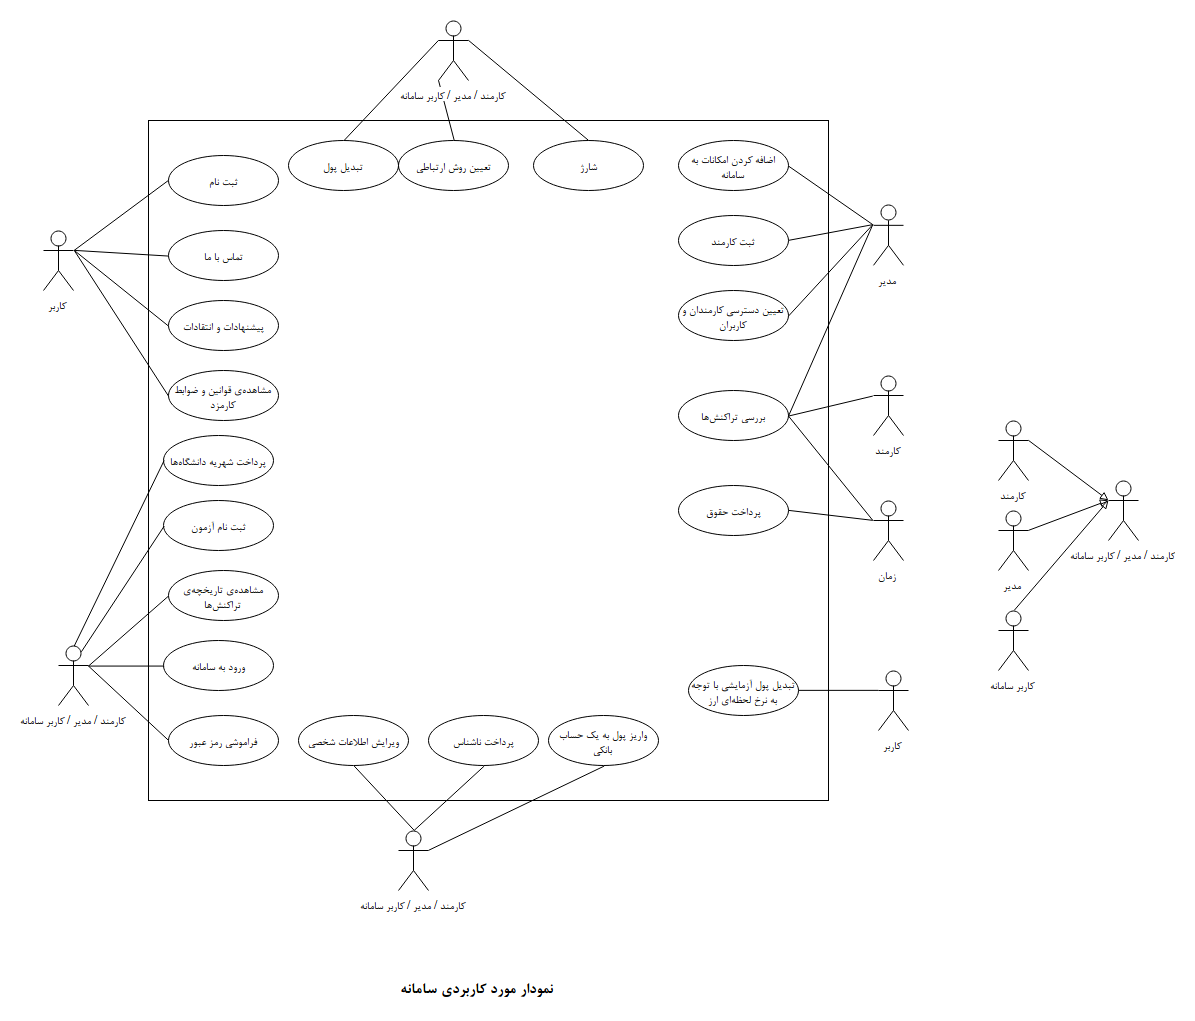
\includegraphics[width = 1\textwidth]{Usecase_Diagram.png}

\section{توضیحات موارد کاربرد}

\begin{table}[h!]
\centering
\begin{tabular}{| c | c |} 
 \hline
\multicolumn{2}{|r|}{\textbf{ثبت‌نام}} \\
 \hline
\textbf{شناسه} &
1 \\
 \hline
 \textbf{توضیح اجمالی}
 &
 یک کاربر سامانه‌ی جدید در سیستم ثبت می‌شود. \\
 \hline
 \textbf{کنشگر اصلی}
 &
 کاربر \\
 \hline
 \textbf{کنشگر فرعی}
 &
  ندارد\\
 \hline
  \textbf{شرایط اولیه}
 &
 کاربر وارد صفحه‌ی ثبت‌نام در سامانه می‌شود. \\
 \hline
  \textbf{روند اصلی}
 &
\begin{tabular}{p{0.8\textwidth}@{}c@{}}
کاربر با پر کردن فرم ثبت‌نام و زدن دکمه‌ی \lr{register} در سیستم ثبت می‌شود.\\
فرم ثبت‌نام شامل موارد زیر است:\\
\begin{itemize}
\item 
ایمیل
\item
رمزعبور و تکرار آن
\item
نام و نام‌خانوادگی
\item
نام کاربری
\item
آدرس
\item
captcha
\item
شماره‌ی ملی
\item
شماره همراه
\end{itemize}
\end{tabular}
\\
\hline
  \textbf{شرایط پایانی}
 &
 کاربر سامانه‌ای با مشخصات وارد شده در فرم در سامانه ثبت‌نام می‌شود. \\
 \hline
  \textbf{سناریوی‌ فرعی}
 &
\begin{tabular}{p{0.8\textwidth}@{}c@{}}
\begin{itemize}
\item
هیچ‌کدام از فیلد‌های فرم نمی‌تواند خالی باشد و در صورت خالی بودن حتی یکی از فیلدها سیستم پیام خطای مربوطه را به کاربر اعلام می‌کند.
\item
رایانامه باید فرمتی درست داشته باشد و در صورت وجود اشکال در فرمت رایانامه سیستم پیام مربوطه را به کاربر اعلام می‌کند.
\item
رمز عبور و تکرار آن باید با یکدیگر مطابقت داشته باشند و در صورت عدم تطابق سیستم پیام مناسب به کاربر اعلام می‌کند.
\item
نام کاربری هر کاربر یکتاست و در صورت استفاده‌ی کاربر دیگری از نام کاربری پیشنهادی سیستم پیام مناسب به کاربر نشان می‌دهد.
\item
\lr{captcha}
ای که توسط کاربر وارد می‌شود باید با آن‌چه در تصویر نشان داده می‌شود،‌ مطابق باشد. در غیر این صورت پیام خطای مناسبی به کاربر نمایش داده می‌شود.
\item
شماره ملی باید اندازه‌ای درست (۱۰ رقم) و فرمتی مناسب داشته باشد در غیر این صورت سیستم پیام مناسب را به کاربر می‌دهد.
\item
شماره‌ی تلفن همراه باید اندازه و فرمتی مناسب داشته باشد در غیر این صورت سیستم پیام مناسب را به کاربر می‌دهد.
\item
در صورت وارد کردن دستورات SQL سیستم به کاربر پیام خطای مناسب را می‌دهد.
\end{itemize}
\end{tabular}
\\
 \hline
\end{tabular}
\caption{ثبت ‌نام}
\label{table:1}
\end{table}

\begin{table}[h!]
\centering
\begin{tabular}{| c | c |} 
 \hline
\multicolumn{2}{|r|}{\textbf{تماس با ما}} \\
 \hline
\textbf{شناسه} &
۲ \\
 \hline
 \textbf{توضیح اجمالی}
 &
کاربر می‌تواند برای سامانه پیام بگذارد. \\
 \hline
 \textbf{کنشگر اصلی}
 &
 کاربر \\
 \hline
 \textbf{کنشگر فرعی}
 &
  ندارد\\
 \hline
  \textbf{شرایط اولیه}
 &
 کاربر وارد صفحه‌ی تماس با ما می‌شود.\\
 \hline
  \textbf{روند اصلی}
 &
\begin{tabular}{p{0.8\textwidth}@{}c@{}}
کاربر با پر کردن فرم تماس با ما و زدن دکمه‌ی \lr{register} در پیام خود را در سیستم ثبت می‌کند.\\
فرم تماس با ما شامل موارد زیر است:\\
\begin{itemize}
\item 
ایمیل
\item
نام و نام‌خانوادگی
\item
نام کاربری
\item
captcha
\item
شماره همراه
\item
متن پیام
\end{itemize}
\end{tabular}
\\
\hline
  \textbf{شرایط پایانی}
 &
 پیام کاربر در سیستم ثبت می‌شود. \\
 \hline
  \textbf{سناریوی‌ فرعی}
 &
\begin{tabular}{p{0.8\textwidth}@{}c@{}}
\begin{itemize}
\item
فیلدهای \lr{captcha} و متن پیام نمی‌توانند خالی باشند.
\item
رایانامه باید فرمتی درست داشته باشد و در صورت وجود اشکال در فرمت رایانامه سیستم پیام مربوطه را به کاربر اعلام می‌کند.
\item
نام کاربری که از آن استفاده می‌شود باید یک نام کاربری ثبت شده در سیستم باشد.
\item
\lr{captcha}
ای که توسط کاربر وارد می‌شود باید با آن‌چه در تصویر نشان داده می‌شود،‌ مطابق باشد. در غیر این صورت پیام خطای مناسبی به کاربر نمایش داده می‌شود.
\item
شماره‌ی تلفن همراه باید اندازه و فرمتی مناسب داشته باشد در غیر این صورت سیستم پیام مناسب را به کاربر می‌دهد.
\item
در صورت وارد کردن دستورات SQL سیستم به کاربر پیام خطای مناسب را می‌دهد.
\end{itemize}
\end{tabular}
\\
 \hline
\end{tabular}
\caption{تماس با ما}
\label{table:1}
\end{table}


\begin{table}[h!]
\centering
\begin{tabular}{| c | c |} 
 \hline
\multicolumn{2}{|r|}{\textbf{ورود به سامانه}} \\
 \hline
\textbf{شناسه} &
۳ \\
 \hline
 \textbf{توضیح اجمالی}
 &
کاربر سامانه /کارمند/مدیر می‌توانند به صفحه‌ی خود وارد شوند.\\
 \hline
 \textbf{کنشگر اصلی}
 &
 کاربر سامانه  - کارمند - مدیر \\
 \hline
 \textbf{کنشگر فرعی}
 &
  ندارد\\
 \hline
  \textbf{شرایط اولیه}
 &
کاربر سامانه /کارمند/مدیر به صفحه‌ی ورود به سایت وارد می‌شوند.\\
 \hline
  \textbf{روند اصلی}
 &
\begin{tabular}{p{0.8\textwidth}@{}c@{}}
کاربر سامانه /کارمند/مدیر با وارد کردن نام کابری و رمز و \lr{captcha} و زدن دکمه‌ی \lr{login} به صفحه‌ی خود در سیستم وارد می‌شوند. در صورتی که رمز عبور فراموش شده باشد، دکمه‌ی فراموشی رمز عبور فشرده می‌شود.
\end{tabular}
\\
\hline
  \textbf{شرایط پایانی}
 &
 \begin{tabular}{p{0.8\textwidth}@{}c@{}}
کاربر/مدیر/کارمند به صفحه‌ی شخصی خود وارد می‌شوند یا در صورت فراموشی رمز عبور به صفحه‌ی فراموشی رمز عبور به صفحه‌ی فراموشی رمز عبور وارد می‌شوند.
\end{tabular}
\\
\hline
  \textbf{سناریوی‌ فرعی}
 &
\begin{tabular}{p{0.8\textwidth}@{}c@{}}
\begin{itemize}
\item
هیچ یک از فیلدها نمی‌توانند خالی باشند.
\item
در صورت اشتباه وارد شدن نام کاربری یا رمزعبور به کاربر پیام مناسب داده خواهد شد.
\item
\lr{captcha}
ای که توسط کاربر وارد می‌شود باید با آن‌چه در تصویر نشان داده می‌شود،‌ مطابق باشد. در غیر این صورت پیام خطای مناسبی به کاربر نمایش داده می‌شود.
\item
در صورت وارد کردن دستورات SQL سیستم به کاربر پیام خطای مناسب را می‌دهد.
\end{itemize}
\end{tabular}
\\
 \hline
\end{tabular}
\caption{ورود به سیستم}
\label{table:1}
\end{table}

\begin{table}[h!]
\centering
\begin{tabular}{| c | c |} 
 \hline
\multicolumn{2}{|r|}{\textbf{فراموشی رمز عبور}} \\
 \hline
\textbf{شناسه} &
۴ \\
 \hline
 \textbf{توضیح اجمالی}
 &
کاربر سامانه /کارمند/مدیر می‌توانند در صورت فراموشی رمز آن را در این صفحه بازیابی کنند.\\
 \hline
 \textbf{کنشگر اصلی}
 &
 کاربر سامانه - کارمند - مدیر \\
 \hline
 \textbf{کنشگر فرعی}
 &
  ندارد\\
 \hline
  \textbf{شرایط اولیه}
 &
کاربر سامانه /کارمند/مدیر به صفحه‌ی فراموشی رمز عبور در سایت وارد می‌شوند.\\
 \hline
  \textbf{روند اصلی}
 &
\begin{tabular}{p{0.8\textwidth}@{}c@{}}
کاربر سامانه /کارمند/مدیر ابتدا نحوه‌ی بازیابی را که می‌تواند از طریق تلگرام، پیامک یا ایمیل باشد را انتخاب می‌کنند. سپس شماره تلفن و رایانامه‌اش را وارد می‌کند. در نهایت با وارد کردن captcha و زدن دکمه‌ی submit می‌تواند رمز خود را بازیابی کند.
\end{tabular}
\\
\hline
  \textbf{شرایط پایانی}
 &
 \begin{tabular}{p{0.8\textwidth}@{}c@{}}
کاربر سامانه /مدیر/کارمند رمز عبور خود را بازیابی می‌کند.
\end{tabular}
\\
\hline
  \textbf{سناریوی‌ فرعی}
 &
\begin{tabular}{p{0.8\textwidth}@{}c@{}}
\begin{itemize}
\item
هیچ یک از فیلدها نمی‌توانند خالی باشند. همچنین حتما باید یکی از ۳ گزینه‌ی ارتباطی انتخاب شده باشد.
\item
فرمت رایانامه باید درست باشد.
\item
\lr{captcha}
ای که توسط کاربر وارد می‌شود باید با آن‌چه در تصویر نشان داده می‌شود،‌ مطابق باشد. در غیر این صورت پیام خطای مناسبی به کاربر نمایش داده می‌شود.
\item
در صورت وارد کردن دستورات SQL سیستم به کاربر پیام خطای مناسب را می‌دهد.
\item
شماره‌ی همراه باید فرمت و اندازه‌ی مناسب داشته باشد.
\end{itemize}
\end{tabular}
\\
 \hline
\end{tabular}
\caption{فراموشی رمز عبور}
\label{table:1}
\end{table}

\begin{table}[h!]
\centering
\begin{tabular}{| c | c |} 
 \hline
\multicolumn{2}{|r|}{\textbf{انتقادات و پیشنهادات}} \\
 \hline
\textbf{شناسه} &
۵ \\
 \hline
 \textbf{توضیح اجمالی}
 &
کاربر می‌تواند انتقادات و پیشنهادات خود را در سیستم ثبت کند.\\
 \hline
 \textbf{کنشگر اصلی}
 &
 کاربر \\
 \hline
 \textbf{کنشگر فرعی}
 &
  ندارد\\
 \hline
  \textbf{شرایط اولیه}
 &
کاربر وارد صفحه‌ی انتقادات و پیشنهادات در سایت وارد می‌شوند.\\
 \hline
  \textbf{روند اصلی}
 &
\begin{tabular}{p{0.8\textwidth}@{}c@{}}
کاربر با نوشتن نام و نام‌خانوادگی، رایانامه، عنوان و متن پیام، شماره همراه، captcha و در نهایت زدن دکمه‌ی register  انتقاد یا پیشنهاد خود را در سیستم ثبت می‌کند.
\end{tabular}
\\
\hline
  \textbf{شرایط پایانی}
 &
 \begin{tabular}{p{0.8\textwidth}@{}c@{}}
پیام کاربر در سیستم ثبت می‌شود.
\end{tabular}
\\
\hline
  \textbf{سناریوی‌ فرعی}
 &
\begin{tabular}{p{0.8\textwidth}@{}c@{}}
\begin{itemize}
\item
رایانامه، عنوان، متن و captcha نمی‌توانند خالی باشد.
\item
فرمت رایانامه باید درست باشد.
\item
\lr{captcha}
ای که توسط کاربر وارد می‌شود باید با آن‌چه در تصویر نشان داده می‌شود،‌ مطابق باشد. در غیر این صورت پیام خطای مناسبی به کاربر نمایش داده می‌شود.
\item
در صورت وارد کردن دستورات SQL سیستم به کاربر پیام خطای مناسب را می‌دهد.
\item
شماره‌ی همراه باید فرمت و اندازه‌ی مناسب داشته باشد.
\end{itemize}
\end{tabular}
\\
 \hline
\end{tabular}
\caption{انتقادات و پیشنهادات}
\label{table:1}
\end{table}


\begin{table}[h!]
\centering
\begin{tabular}{| c | c |} 
 \hline
\multicolumn{2}{|r|}{\textbf{شارژ}} \\
 \hline
\textbf{شناسه} &
۶ \\
 \hline
 \textbf{توضیح اجمالی}
 &
کاربر سامانه/مدیر/ کارمند می‌تواند حساب خود را شارژ کند. (مدیر حساب سامانه را هم می‌تواند شارژ می‌کند)\\
 \hline
 \textbf{کنشگر اصلی}
 &
 کاربر سامانه / مدیر / کارمند \\
 \hline
 \textbf{کنشگر فرعی}
 &
  ندارد\\
 \hline
  \textbf{شرایط اولیه}
 &
کاربر سامانه / مدیر / کارمند وارد صفحه‌ی شخصی خود در سامانه شوند.\\
 \hline
  \textbf{روند اصلی}
 &
\begin{tabular}{p{0.8\textwidth}@{}c@{}}
کاربر سامانه/مدیر / کارمند  با زدن دکمه‌ی شارژ در صفحه‌ی خود و انتخاب مبلغ مورد نظر و زدن دکمه‌ی خرید حساب خود را شارژ می‌کنند. مدیر حساب سامانه را هم می‌تواند شارژ کند.
\end{tabular}
\\
\hline
  \textbf{شرایط پایانی}
 &
 \begin{tabular}{p{0.8\textwidth}@{}c@{}}
مبلغ شارژ شده به حساب سامانه/کاربر واریز می‌شود. همچنین رسید تراکنش از طریقی که کاربر انتخاب کرده به او ارسال می‌گردد.
\end{tabular}
\\
\hline
  \textbf{سناریوی‌ فرعی}
 &
\begin{tabular}{p{0.8\textwidth}@{}c@{}}
\begin{itemize}
\item
مبلغ نمی‌تواند از یک حدی کمتر یا بیشتر باشد، همچنین حتما باید عددی باشد.
\item
مبلغ نمی‌تواند خالی باشد.
\end{itemize}
\end{tabular}
\\
 \hline
\end{tabular}
\caption{شارژ}
\label{table:1}
\end{table}

\begin{table}[h!]
\centering
\begin{tabular}{| c | c |} 
 \hline
\multicolumn{2}{|r|}{\textbf{ویرایش اطلاعات شخصی}} \\
 \hline
\textbf{شناسه} &
۷ \\
 \hline
 \textbf{توضیح اجمالی}
 &
کاربر سامانه/مدیر / کارمند می‌تواند اطلاعات شخصی خود در سامانه را ویرایش کند.\\
 \hline
 \textbf{کنشگر اصلی}
 &
کارمند / کاربر سامانه / مدیر \\
 \hline
 \textbf{کنشگر فرعی}
 &
  ندارد\\
 \hline
  \textbf{شرایط اولیه}
 &
کاربر سامانه / مدیر / کاربر وارد صفحه‌ی مشاهده‌ی اطلاعات شخصی خود در سامانه شوند.\\
 \hline
  \textbf{روند اصلی}
 &
\begin{tabular}{p{0.8\textwidth}@{}c@{}}
کارمند / کاربر سامانه/مدیر می‌توانند برخی اطلاعات شخصی خود مانند شماره همراه، آواتار، رمز عبور یا رایانامه‌ی خود را ویرایش کنند.
\end{tabular}
\\
\hline
  \textbf{شرایط پایانی}
 &
 \begin{tabular}{p{0.8\textwidth}@{}c@{}}
اطلاعات شخصی جدید در صورت درست بودن در سامانه بروز می‌شوند.
\end{tabular}
\\
\hline
  \textbf{سناریوی‌ فرعی}
 &
\begin{tabular}{p{0.8\textwidth}@{}c@{}}
\begin{itemize}
\item
شماره تلفن باید فرمت و اندازه‌ی مناسب داشته باشد.
\item
رایانامه باید فرمت درستی داشته باشد.
\item
رمز عبور و تکرار آن باید تطابق داشته باشند.
\item
در صورت استفاده از دستورات SQL سیستم پیام خطای مناسب را به کاربر نمایش می‌دهد.
\end{itemize}
\end{tabular}
\\
 \hline
\end{tabular}
\caption{ویرایش اطلاعات شخصی}
\label{table:1}
\end{table}

\begin{table}[h!]
\centering
\begin{tabular}{| c | c |} 
 \hline
\multicolumn{2}{|r|}{\textbf{مشاهده‌ی تارخچه‌ی تراکنش‌ها}} \\
 \hline
\textbf{شناسه} &
۸ \\
 \hline
 \textbf{توضیح اجمالی}
 &
کاربر سامانه / مدیر / کارمند می‌توانند تاریخچه‌ی تراکنش‌هایی که در سامانه انجام داده اند را مشاهده کنند.\\
 \hline
 \textbf{کنشگر اصلی}
 &
کارمند / کاربر سامانه / مدیر \\
 \hline
 \textbf{کنشگر فرعی}
 &
ندارد\\
 \hline
  \textbf{شرایط اولیه}
 &
کاربر سامانه / مدیر / کاربر وارد صفحه‌ی مشاهده‌ی تاریخچه‌ی تراکنش خود در سامانه شوند.\\
 \hline
  \textbf{روند اصلی}
 &
\begin{tabular}{p{0.8\textwidth}@{}c@{}}
در این صفحه جدولی از خلاصه‌ی تراکنش‌های انجام شده برای شخص نمایش داده خواهد شد و می‌تواند با جستجو تراکنش مورد نظر خود را بیابد.
\end{tabular}
\\
\hline
  \textbf{شرایط پایانی}
 &
 \begin{tabular}{p{0.8\textwidth}@{}c@{}}
ندارد.
\end{tabular}
\\
\hline
  \textbf{سناریوی‌ فرعی}
 &
\begin{tabular}{p{0.8\textwidth}@{}c@{}}
ندارد
\end{tabular}
\\
 \hline
\end{tabular}
\caption{مشاهده‌ی تاریخچه‌ی تراکنش‌ها}
\label{table:1}
\end{table}


\begin{table}[h!]
\centering
\begin{tabular}{| c | c |} 
 \hline
\multicolumn{2}{|r|}{\textbf{مشاهده‌ی قوانین ضوابط و کارمزد}} \\
 \hline
\textbf{شناسه} &
۹ \\
 \hline
 \textbf{توضیح اجمالی}
 &
کاربر می‌تواند از قوانین و ضوابط و کارمزد خدمات گوناگون در سامانه مطلع شود.\\
 \hline
 \textbf{کنشگر اصلی}
 &
کاربر \\
 \hline
 \textbf{کنشگر فرعی}
 &
  ندارد\\
 \hline
  \textbf{شرایط اولیه}
 &
کاربر به صفحه‌ی قوانین در سایت وارد شود.\\
 \hline
  \textbf{روند اصلی}
 &
\begin{tabular}{p{0.8\textwidth}@{}c@{}}
مطالعیه صفحه‌ی قوانین.
\end{tabular}
\\
\hline
  \textbf{شرایط پایانی}
 &
 \begin{tabular}{p{0.8\textwidth}@{}c@{}}
ندارد.
\end{tabular}
\\
\hline
  \textbf{سناریوی‌ فرعی}
 &
\begin{tabular}{p{0.8\textwidth}@{}c@{}}
ندارد.
\end{tabular}
\\
 \hline
\end{tabular}
\caption{مشاهده‌ی قوانین، ضوابط و کارمزد}
\label{table:1}
\end{table}


\begin{table}[h!]
\centering
\begin{tabular}{| c | c |} 
 \hline
\multicolumn{2}{|r|}{\textbf{پرداخت شهریه‌ی داشنگاه‌ها}} \\
 \hline
\textbf{شناسه} &
۱۰ \\
 \hline
 \textbf{توضیح اجمالی}
 &
کاربر سامانه / مدیر / کارمند می‌تواند به حساب دانشگاه مورد نظر خود پول واریز کند.\\
 \hline
 \textbf{کنشگر اصلی}
 &
کارمند / کاربر سامانه / مدیر \\
 \hline
 \textbf{کنشگر فرعی}
 &
  ندارد\\
 \hline
  \textbf{شرایط اولیه}
 &
کاربر سامانه / مدیر / کاربر وارد صفحه‌ی شخصی خود در سامانه شوند.\\
 \hline
  \textbf{روند اصلی}
 &
\begin{tabular}{p{0.8\textwidth}@{}c@{}}
کارمند / کاربر سامانه/مدیر می‌توانند با وارد کردن شماره حساب و مقدار پولی که می‌خواهند واریز کنند و همچنین نوع ارز، پس از مشاهده‌ی قیمت کارمزد، شهریه‌ی دانشگاه مورد نظر خود را پرداخت نماید. 
\end{tabular}
\\
\hline
  \textbf{شرایط پایانی}
 &
 \begin{tabular}{p{0.8\textwidth}@{}c@{}}
تراکنش انجام می‌گیرد و رسید تراکنش از طریقی که کاربر انتخاب کرده به او اعلام می‌شود.
\end{tabular}
\\
\hline
  \textbf{سناریوی‌ فرعی}
 &
\begin{tabular}{p{0.8\textwidth}@{}c@{}}
\begin{itemize}
\item
مقدار پول در حساب باید برای پرداخت کافی باشد.
\item
شماره‌ی کارت باید اندازه‌ی مناسب داشته باشد.
\item
مبلغ مورد نظر باید از کفی بیشتر و از سقفی کمتر باشد.
\item
انواع مختلف ارز شامل دلار، ریال و یورو است.
\item
در صورت استفاده از دستورات SQL سیستم پیام خطای مناسب را به کاربر نمایش می‌دهد.
\end{itemize}
\end{tabular}
\\
 \hline
\end{tabular}
\caption{پرداخت شهریه‌ی دانشگاه‌ها}
\label{table:1}
\end{table}

\begin{table}[h!]
\centering
\begin{tabular}{| c | c |} 
 \hline
\multicolumn{2}{|r|}{\textbf{ثبت نام آزمون‌های مختلف}} \\
 \hline
\textbf{شناسه} &
۱۱ \\
 \hline
 \textbf{توضیح اجمالی}
 &
کاربر سامانه / مدیر / کارمند می‌تواند در آزمون‌های مختلف بین‌المللی ثبت نام کند.\\
 \hline
 \textbf{کنشگر اصلی}
 &
کارمند / کاربر سامانه / مدیر \\
 \hline
 \textbf{کنشگر فرعی}
 &
  ندارد\\
 \hline
  \textbf{شرایط اولیه}
 &
کاربر سامانه / مدیر / کاربر وارد صفحه‌ی شخصی خود در سامانه شوند.\\
 \hline
  \textbf{روند اصلی}
 &
\begin{tabular}{p{0.8\textwidth}@{}c@{}}
کارمند / کاربر سامانه/مدیر می‌توانند در صورت داشتن موجودی در کیف پول مورد نظر پس از مشاهده‌ی قیمت کل آزمون،‌مبلغی که لازم است را برای شرکت در آن آزمون پرداخت نماید.
\end{tabular}
\\
\hline
  \textbf{شرایط پایانی}
 &
 \begin{tabular}{p{0.8\textwidth}@{}c@{}}
تراکنش انجام می‌گیرد و رسید تراکنش از طریقی که کاربر انتخاب کرده به او اعلام می‌شود.
\end{tabular}
\\
\hline
  \textbf{سناریوی‌ فرعی}
 &
\begin{tabular}{p{0.8\textwidth}@{}c@{}}
\begin{itemize}
\item
مقدار پول در حساب باید برای ثبت‌نام در آزمون کافی باشد.
\end{itemize}
\end{tabular}
\\
 \hline
\end{tabular}
\caption{ثبت نام در آزمون‌های بین‌المللی}
\label{table:1}
\end{table}


\begin{table}[h!]
\centering
\begin{tabular}{| c | c |} 
 \hline
\multicolumn{2}{|r|}{\textbf{پرداخت ناشناس}} \\
 \hline
\textbf{شناسه} &
۱۲ \\
 \hline
 \textbf{توضیح اجمالی}
 &
کاربر سامانه / مدیر / کارمند می‌تواند به صورت ناشناس به حساب شخص دیگری واریز داشته باشند.\\
 \hline
 \textbf{کنشگر اصلی}
 &
کارمند / کاربر سامانه / مدیر \\
 \hline
 \textbf{کنشگر فرعی}
 &
  ندارد\\
 \hline
  \textbf{شرایط اولیه}
 &
کاربر سامانه / مدیر / کاربر وارد صفحه‌ی شخصی خود در سامانه شوند.\\
 \hline
  \textbf{روند اصلی}
 &
\begin{tabular}{p{0.8\textwidth}@{}c@{}}
کارمند / کاربر سامانه/مدیر می‌توانند در صورت داشتن موجودی از نوع ارز مورد نظر با دادن شماره‌ی حساب شخص مورد نظر و مبلغ واریزی پس از مشاهده‌ی کارمزد به شماره حساب مورد نظر پول واریز کند.

اگر شخص مورد نظر در سامانه وجود نداشت برای او یک حساب کاربری ساخته می‌شود و به حساب او پول ریخته می‌شود.
\end{tabular}
\\
\hline
  \textbf{شرایط پایانی}
 &
 \begin{tabular}{p{0.8\textwidth}@{}c@{}}
تراکنش انجام می‌گیرد و رسید تراکنش از طریقی که کاربر انتخاب کرده به او اعلام می‌شود.
\end{tabular}
\\
\hline
  \textbf{سناریوی‌ فرعی}
 &
\begin{tabular}{p{0.8\textwidth}@{}c@{}}
\begin{itemize}
\item
مقدار پول در حساب باید برای واریز کافی باشد.
\item
مبلغ تراکنش باید در محدوده‌ی مجاز در سامانه باشد.
\item
انواع مختلف ارز شامل فقط و فقط ریال، دلار و یورو است.
\item
در صورت استفاده از دستورات SQL سیستم پیام مناسب این خطا را به کاربر می‌دهد.
\end{itemize}
\end{tabular}
\\
 \hline
\end{tabular}
\caption{پرداخت ناشناس}
\label{table:1}
\end{table}




\begin{table}[h!]
\centering
\begin{tabular}{| c | c |} 
 \hline
\multicolumn{2}{|r|}{\textbf{واریز پول به یک حساب بانکی خارجی}} \\
 \hline
\textbf{شناسه} &
۱۳ \\
 \hline
 \textbf{توضیح اجمالی}
 &
کاربر سامانه / مدیر / کارمند می‌تواند به حسابی در خارج از کشور پول واریز کند.\\
 \hline
 \textbf{کنشگر اصلی}
 &
کارمند / کاربر سامانه / مدیر \\
 \hline
 \textbf{کنشگر فرعی}
 &
  ندارد\\
 \hline
  \textbf{شرایط اولیه}
 &
کاربر سامانه / مدیر / کاربر وارد صفحه‌ی شخصی خود در سامانه شوند.\\
 \hline
  \textbf{روند اصلی}
 &
\begin{tabular}{p{0.8\textwidth}@{}c@{}}
کارمند / کاربر سامانه/مدیر می‌توانند در صورت داشتن موجودی از نوع ارز مورد نظر با دادن شماره‌ی حساب شخص مورد نظر و مبلغ واریزی پس از مشاهده‌ی کارمزد به شماره حساب مورد نظر پول واریز کند.
\end{tabular}
\\
\hline
  \textbf{شرایط پایانی}
 &
 \begin{tabular}{p{0.8\textwidth}@{}c@{}}
تراکنش انجام می‌گیرد و رسید تراکنش از طریقی که کاربر انتخاب کرده به او اعلام می‌شود.
\end{tabular}
\\
\hline
  \textbf{سناریوی‌ فرعی}
 &
\begin{tabular}{p{0.8\textwidth}@{}c@{}}
\begin{itemize}
\item
مقدار پول در حساب باید برای واریز کافی باشد.
\item
مبلغ تراکنش باید در محدوده‌ی مجاز در سامانه باشد.
\item
انواع مختلف ارز شامل فقط و فقط ریال، دلار و یورو است.
\item
در صورت استفاده از دستورات SQL سیستم پیام مناسب این خطا را به کاربر می‌دهد.
\end{itemize}
\end{tabular}
\\
 \hline
\end{tabular}
\caption{واریز پول به یک حساب بانکی خارجی}
\label{table:1}
\end{table}



\begin{table}[h!]
\centering
\begin{tabular}{| c | c |} 
 \hline
\multicolumn{2}{|r|}{\textbf{تبدیل پول آزمایشی}} \\
 \hline
\textbf{شناسه} &
۱۴ \\
 \hline
 \textbf{توضیح اجمالی}
 &
\begin{tabular}{p{0.8\textwidth}@{}c@{}}
انجام تبدیلات بین ارزهای مختلف.
\end{tabular}
\\
\hline
 \textbf{کنشگر اصلی}
 &
کاربر \\
 \hline
 \textbf{کنشگر فرعی}
 &
  ندارد\\
 \hline
  \textbf{شرایط اولیه}
 &
دسترسی به سامانه فراهم باشد.\\
 \hline
  \textbf{روند اصلی}
 &
\begin{tabular}{p{0.8\textwidth}@{}c@{}}
کاربر می‌تواند نرخ لحظه‌ای ارز را مشاهده کند و با توجه به آن تبدیلات مالی مختلف را انجام دهد.
\end{tabular}
\\
\hline
  \textbf{شرایط پایانی}
 &
 \begin{tabular}{p{0.8\textwidth}@{}c@{}}
ندارد.
\end{tabular}
\\
\hline
  \textbf{سناریوی‌ فرعی}
 &
\begin{tabular}{p{0.8\textwidth}@{}c@{}}
ندارد.
\end{tabular}
\\
 \hline
\end{tabular}
\caption{تبدیل پول آزمایشی}
\label{table:1}
\end{table}


\begin{table}[h!]
\centering
\begin{tabular}{| c | c |} 
 \hline
\multicolumn{2}{|r|}{\textbf{پرداخت حقوق}} \\
 \hline
\textbf{شناسه} &
۱۵ \\
 \hline
 \textbf{توضیح اجمالی}
 &
پرداخت حقوق به کارمندان.\\
 \hline
 \textbf{کنشگر اصلی}
 &
زمان \\
 \hline
 \textbf{کنشگر فرعی}
 &
  ندارد\\
 \hline
  \textbf{شرایط اولیه}
 &
ندارد.\\
 \hline
  \textbf{روند اصلی}
 &
\begin{tabular}{p{0.8\textwidth}@{}c@{}}
در بازه‌های زمانی مشخص به کارمندان در سامانه حقوق پرداخت می‌شود.
\end{tabular}
\\
\hline
  \textbf{شرایط پایانی}
 &
 \begin{tabular}{p{0.8\textwidth}@{}c@{}}
حقوق در کیف پول ریالی کارمندان شارژ می‌شود.
\end{tabular}
\\
\hline
  \textbf{سناریوی‌ فرعی}
 &
\begin{tabular}{p{0.8\textwidth}@{}c@{}}
\begin{itemize}
\item
در صورت نبودن موجودی کافی در حساب سامانه برای پرداخت حقوق کارمندان هشداری به مدیر سایت فرستاده می‌شود.
\end{itemize}
\end{tabular}
\\
 \hline
\end{tabular}
\caption{پرداخت حقوق}
\label{table:1}
\end{table}


\begin{table}[h!]
\centering
\begin{tabular}{| c | c |} 
 \hline
\multicolumn{2}{|r|}{\textbf{بررسی تراکنش‌ها}} \\
 \hline
\textbf{شناسه} &
۱۶ \\
 \hline
 \textbf{توضیح اجمالی}
 &
بررسی تراکنش‌هایی که کاربران سامانه انجام می‌دهند.\\
 \hline
 \textbf{کنشگر اصلی}
 &
کارمند / مدیر \\
 \hline
 \textbf{کنشگر فرعی}
 &
 زمان\\
 \hline
  \textbf{شرایط اولیه}
 &
کارمند/مدیر به صفحه‌ی شخصی خود در سامانه وارد شده باشند.\\
 \hline
  \textbf{روند اصلی}
 &
\begin{tabular}{p{0.8\textwidth}@{}c@{}}
کارمند/مدیر می‌تواند تراکنش‌هایی که در سیستم انجام شده است را با جزئیات آن مشاهده نماید. و آن را تایید یا رد کند همچنین کارمند می‌تواند در صورت مشاهده‌ی امری غیرعادی آن را به مدیر گزارش کند.
\end{tabular}
\\
\hline
  \textbf{شرایط پایانی}
 &
 \begin{tabular}{p{0.8\textwidth}@{}c@{}}
تراکنش انجام یا رد می‌شود که در صورت رد شدن پیامی به مشتری مبتنی بر همین امر ارسال می‌شود.
\end{tabular}
\\
\hline
  \textbf{سناریوی‌ فرعی}
 &
\begin{tabular}{p{0.8\textwidth}@{}c@{}}
\begin{itemize}
\item
در صورت عدم بررسی یک تراکنش تا ۲۴ ساعت این تراکنش به طور خودکار رد خواهد شد و پیامی مبتنی بر رد شدن تراکنش به مشتری فرستاده می‌شود.
\end{itemize}
\end{tabular}
\\
 \hline
\end{tabular}
\caption{بررسی تراکنش‌ها}
\label{table:1}
\end{table}


\begin{table}[h!]
\centering
\begin{tabular}{| c | c |} 
 \hline
\multicolumn{2}{|r|}{\textbf{تعیین دسترسی کارمندان و کاربران سامانه به سیستم}} \\
 \hline
\textbf{شناسه} &
۱۷ \\
 \hline
 \textbf{توضیح اجمالی}
 &
اجازه یا عدم اجازه‌ی دسترسی به سامانه.\\
 \hline
 \textbf{کنشگر اصلی}
 &
مدیر \\
 \hline
 \textbf{کنشگر فرعی}
 &
 ندارد\\
 \hline
  \textbf{شرایط اولیه}
 &
مدیر به صفحه‌ی شخصی خود در سامانه وارد شده باشد.\\
 \hline
  \textbf{روند اصلی}
 &
\begin{tabular}{p{0.8\textwidth}@{}c@{}}
مدیر می‌تواند در صورت مشاهده‌ی تخلف توسط یک کارمند یا کاربر سامانه دسترسی او را به سیستم قطع نماید. یا پس از رفع ابهامات اجازه‌ی دسترسی کسی را که دسترسی‌اش قطع شده، بدهد.
\end{tabular}
\\
\hline
  \textbf{شرایط پایانی}
 &
 \begin{tabular}{p{0.8\textwidth}@{}c@{}}
دسترسی فرد به سیستم قطع یا وصل می‌شود.
\end{tabular}
\\
\hline
  \textbf{سناریوی‌ فرعی}
 &
\begin{tabular}{p{0.8\textwidth}@{}c@{}}
ندارد.
\end{tabular}
\\
 \hline
\end{tabular}
\caption{تعیین دسترسی کارمندان و کاربران سامانه}
\label{table:1}
\end{table}



\begin{table}[h!]
\centering
\begin{tabular}{| c | c |} 
 \hline
\multicolumn{2}{|r|}{\textbf{ثبت کارمندان}} \\
 \hline
\textbf{شناسه} &
۱۸ \\
 \hline
 \textbf{توضیح اجمالی}
 &
استخدام کارمند.\\
 \hline
 \textbf{کنشگر اصلی}
 &
مدیر \\
 \hline
 \textbf{کنشگر فرعی}
 &
 ندارد.\\
 \hline
  \textbf{شرایط اولیه}
 &
مدیر به صفحه‌ی شخصی خود در سامانه وارد شده باشد.\\
 \hline
  \textbf{روند اصلی}
 &
\begin{tabular}{p{0.8\textwidth}@{}c@{}}
مدیر می‌تواند با افزودن مشخصات یک کارمند که دقیقا همانند مشخصات یک کاربر سامانه است (ر.ک. به مورد کاربردی ثبت نام در سامانه) و مشخص کردن حقوق او. یک کاربر را در سامانه استخدام کند.
\end{tabular}
\\
\hline
  \textbf{شرایط پایانی}
 &
 \begin{tabular}{p{0.8\textwidth}@{}c@{}}
مشخصات کارمند در سامانه ثبت می‌شود.
\end{tabular}
\\
\hline
  \textbf{سناریوی‌ فرعی}
 &
\begin{tabular}{p{0.8\textwidth}@{}c@{}}
ر.ک. به سناریوی فرعی مورد کاربردی ثبت‌نام 
\end{tabular}
\\
 \hline
\end{tabular}
\caption{استخدام کارمندان}
\label{table:1}
\end{table}


\begin{table}[h!]
\centering
\begin{tabular}{| c | c |} 
 \hline
\multicolumn{2}{|r|}{\textbf{اضافه کردن امکانات به سامانه}} \\
 \hline
\textbf{شناسه} &
۱۹ \\
 \hline
 \textbf{توضیح اجمالی}
 &
افزودن آزمون جدید به سامانه.\\
 \hline
 \textbf{کنشگر اصلی}
 &
مدیر \\
 \hline
 \textbf{کنشگر فرعی}
 &
 ندارد.\\
 \hline
  \textbf{شرایط اولیه}
 &
مدیر به صفحه‌ی شخصی خود در سامانه وارد شده باشد.\\
 \hline
  \textbf{روند اصلی}
 &
\begin{tabular}{p{0.8\textwidth}@{}c@{}}
مدیر می‌تواند آزمون جدیدی را در سامانه تعریف کند. این آزمون در بخش ثبت‌نام در آزمون‌های بین‌المللی افزوده می‌شود. برای این کار باید:
\begin{itemize}
\item
نام آزمون
\item
مبلغ آزمون
\item
کارمزدی که برای ثبت‌نام در آن دریافت می‌شود.
\item
تاریخ آزمون
\end{itemize}
وارد سامانه شود.
\end{tabular}
\\
\hline
  \textbf{شرایط پایانی}
 &
 \begin{tabular}{p{0.8\textwidth}@{}c@{}}
آزمون جدید به بخش آزمون‌ها در سامانه افزوده می‌شود.
\end{tabular}
\\
\hline
  \textbf{سناریوی‌ فرعی}
 &
\begin{tabular}{p{0.8\textwidth}@{}c@{}}
\begin{itemize}
\item
تاریخ آزمون باید مربوط به آینده باشد.
\end{itemize}
\end{tabular}
\\
 \hline
\end{tabular}
\caption{اضافه‌کردن امکانات به سامانه}
\label{table:1}
\end{table}


\begin{table}[h!]
\centering
\begin{tabular}{| c | c |} 
 \hline
\multicolumn{2}{|r|}{\textbf{تعیین روش ارتباطی}} \\
 \hline
\textbf{شناسه} &
۲۰ \\
 \hline
 \textbf{توضیح اجمالی}
 &
تعیین روش ارتباطی سامانه با کاربرسامانه / مدیر / کارمند.\\
 \hline
 \textbf{کنشگر اصلی}
 &
کاربر سامانه / مدیر / کارمند \\
 \hline
 \textbf{کنشگر فرعی}
 &
 ندارد.\\
 \hline
  \textbf{شرایط اولیه}
 &
مدیر / کاربر سامانه / کارمند  به صفحه‌ی شخصی خود در سامانه وارد شده باشد.\\
 \hline
  \textbf{روند اصلی}
 &
\begin{tabular}{p{0.8\textwidth}@{}c@{}}
افراد می‌توانند روش ارتباطی خود و سامانه را بین روش های پیامکی، ایمیل و تلگرام انتخاب کنند.
\end{tabular}
\\
\hline
  \textbf{شرایط پایانی}
 &
 \begin{tabular}{p{0.8\textwidth}@{}c@{}}
روش ارتباطی فرد با سامانه در سیستم مشخص می‌گردد.
\end{tabular}
\\
\hline
  \textbf{سناریوی‌ فرعی}
 &
\begin{tabular}{p{0.8\textwidth}@{}c@{}}
\begin{itemize}
\item
فرمت رایانامه باید درست باشد.
\item
فرمت و اندازه‌ی شماره‌ی تلفن باید درست باشد.
\item
در صورت انتخاب بات تلگرام برای ارتباط باید مقدمه‌ی این ارتباط توسط کاربر فراهم شود.
\end{itemize}
\end{tabular}
\\
 \hline
\end{tabular}
\caption{تعیین روش‌ ارتباطی با سامانه}
\label{table:1}
\end{table}


\begin{table}[h!]
\centering
\begin{tabular}{| c | c |} 
 \hline
\multicolumn{2}{|r|}{\textbf{تبدیل پول واقعی}} \\
 \hline
\textbf{شناسه} &
۲۱ \\
 \hline
 \textbf{توضیح اجمالی}
 &
تبدیل ارز‌های مختلف به یکدیگر.\\
 \hline
 \textbf{کنشگر اصلی}
 &
کاربر سامانه / مدیر / کارمند \\
 \hline
 \textbf{کنشگر فرعی}
 &
 ندارد.\\
 \hline
  \textbf{شرایط اولیه}
 &
مدیر / کاربر سامانه / کارمند  به صفحه‌ی شخصی خود در سامانه وارد شده باشد.\\
 \hline
  \textbf{روند اصلی}
 &
\begin{tabular}{p{0.8\textwidth}@{}c@{}}
افراد می‌توانند با توجه به قیمت لحظه‌ای ارزهای گوناگون دارایی‌های کیف پول‌های مختلف خود را به یکدیگر تبدیل کنند. در این تبدیل کارمزدی به حساب سامانه واریز می‌شود.
\end{tabular}
\\
\hline
  \textbf{شرایط پایانی}
 &
 \begin{tabular}{p{0.8\textwidth}@{}c@{}}
ارز مورد نظر تبدیل شده و در حساب شخص لحاظ می‌شود. همچنین رسید تراکنش توسط روش ارتباطی مشخص شده به شخص اعلام می‌شود.
\end{tabular}
\\
\hline
  \textbf{سناریوی‌ فرعی}
 &
\begin{tabular}{p{0.8\textwidth}@{}c@{}}
\begin{itemize}
\item
مبلغ مورد نظر باید در محدوده‌ی مجاز در سامانه باشد.
\end{itemize}
\end{tabular}
\\
 \hline
\end{tabular}
\caption{تبدیل پول‌های مختلف}
\label{table:1}
\end{table}

\end{document} 

